\documentclass{article}
\usepackage{amsmath}
\usepackage{pgfplots}
\pgfplotsset{width=9cm,compat=1.8} 

\title{Isotermas}

\begin{document}
\maketitle

Dada la relación entre la presión, el volumen y la temperatura entre un sistema y el medio
\begin{equation}
    \frac{P_1 V_1}{T_1} = \frac{P_2 V_2}{T_2}
\end{equation}

Tenemos que, en una transformación isotérmica, donde $T_1 = T_2$, la relación
está dada por
\begin{equation}
    P_1 V_1 = P_2 V_2
\end{equation}

Ahora, podemos definir una función $K(p, v)$ dada  $K = p v$, donde $p$ es la presión y $v$ el volumen, y son variables. 

Si despejamos la presión, nos da $p=\frac{K}{v}$, que es una hipérbola equilátera y llamamos a esta función \textit{isoterma}.

En este caso $K$ permanece constante, y como tenemos la siguiente relación
\begin{equation}
    \begin{split}
        v \propto T \\ 
        p \propto T
    \end{split}
\end{equation}
donde $T$ es la temperatura, tenemos que $K \propto T$. De forma que $K$ está ligado directamente a la temperatura (como era de esperar).

\begin{center}
    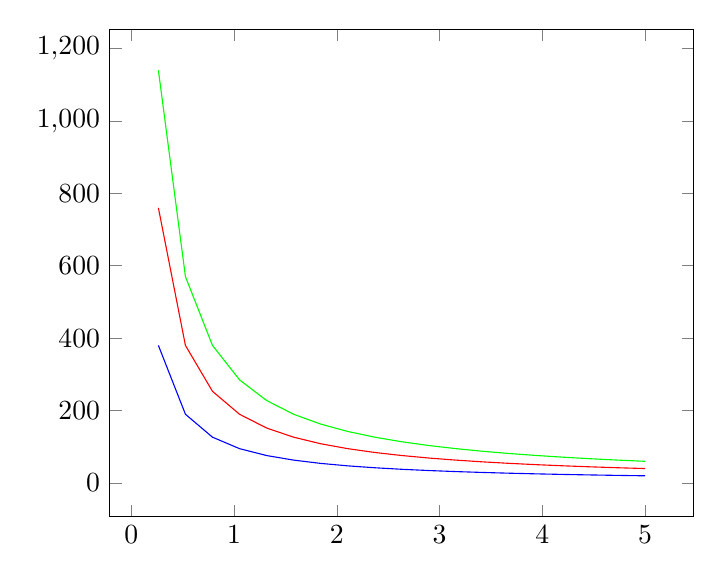
\begin{tikzpicture}
        \begin{axis}
            \addplot[samples=20, color=green, domain=0:5]{300 / x};
            \addplot[samples=20, color=red, domain=0:5]{200 / x};
            \addplot[samples=20, color=blue, domain=0:5]{100 / x};
        \end{axis}
    \end{tikzpicture}
\end{center}

\end{document}
